\documentclass[12pt]{report}
\usepackage[a4paper, left=0.5in, right=0.5in, top=0.5in, bottom=0.5in]{geometry}
\usepackage{xcolor}
\usepackage{amsmath}
\usepackage{amsthm}
\usepackage{amssymb}
\usepackage{amsfonts}
\usepackage{algpseudocode}
\usepackage{mathtools}
\usepackage{xcolor}
\usepackage{float}
\usepackage{framed}
\usepackage{listings}
\usepackage{graphicx}
\usepackage{subcaption}
\usepackage{tikz}
\usepackage{emoji}

\lstset{basicstyle=\ttfamily,
  commentstyle=\color{red},
  keywordstyle=\color{blue},
  %basicstyle=\footnotesize,
  frame=lines,
  numbers=left,
  stepnumber=1,
  showstringspaces=false,
  tabsize=1,
  breaklines=true,
  breakatwhitespace=false,
}
\usepackage{hyperref}
\hypersetup
{
    colorlinks=true,
    linkcolor=blue,
    filecolor=magenta,
    urlcolor=cyan,
    pdftitle={\Huge \textbf{CS218 Solutions Advanced}},
    pdfpagemode=FullScreen,
}
\usepackage[utf8]{inputenc}
\usepackage{graphicx}
\usepackage{longtable}
\usepackage{multirow}
\usepackage{enumitem}
\setlength{\parindent}{0pt}

\begin{document}
\subsection*{\bfseries Linear Programming, Approximation, Randomized, Error correction}
\begin{enumerate}[label=\textbf{\arabic*.}]

    \item If you think about the algorithm, it selects and edge and then deletes the vertices of the edge, so it's going to go over a
    set of disjoint edges with no common vertex. Say it goes of $k$ edges like this. We know that the minimum vertex cover size is at
    least $k$, as we have to select at least one vertex incident to each edge of this set, if not we won't cover the edge. And the
    number of vertices selected by our approximation algo is $2k$, so it is atmost twice the optimal solution.

    It's easy to see that we are basically getting a matching of size $k$ from this algorithm. We now have to prove that the maximum
    matching isn't bigger than $2k$, assume it's actually bigger. This would mean there's a match without having any vertex in the $2k$
    vertex our algorithm returned. Why? Because each of the $2k$ vertex can be in atmost a single match (matches are vertex disjoint).
    But if there's an edge which doesn't have a vertex common with the $2k$ vertices, our algorithm didn't return a vertex cover, which 
    is a contradiction.

    \item Kinda complicated example \emoji{grinning-face-with-sweat}. It's a bipartite graph.
    
    \begin{figure}[H]
        \centering
        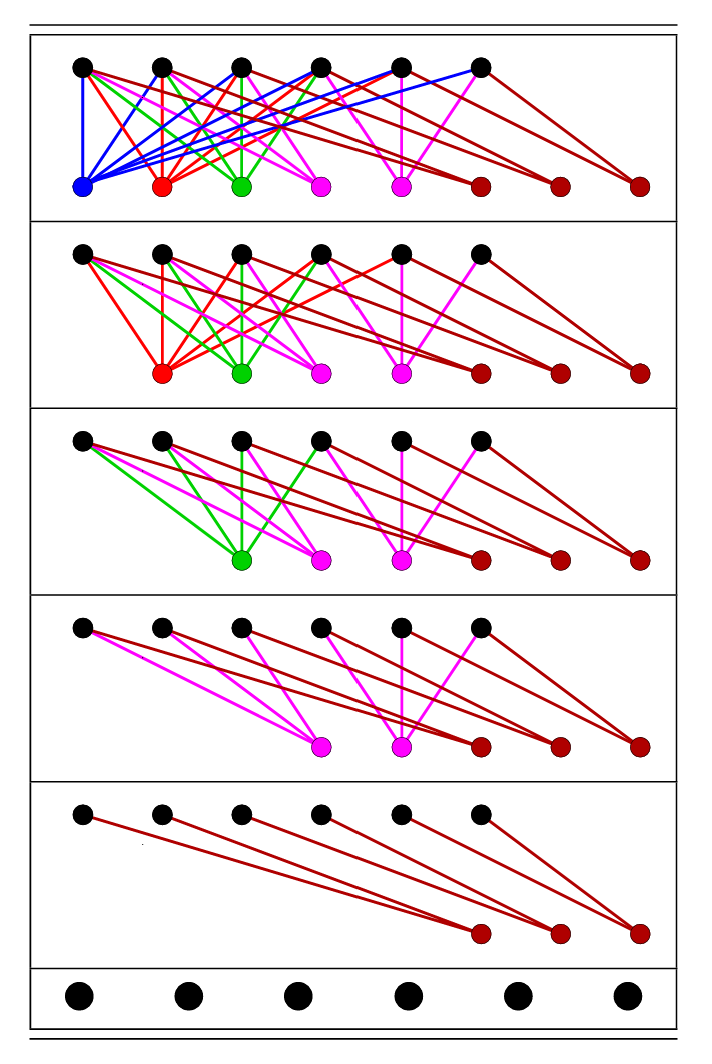
\includegraphics[width=0.5\textwidth]{GreedyVertexCover.png}  
    \end{figure}

    Let the first row of the graph be $n$ vertices, for the figure above it is $n = 6$. For the bottom row, for every $i$ from 2 to $n$, 
    we will have $\lfloor n/i \rfloor$ of degree $i$, each of them connected to distinct vertices in the top row. So in the above figure 
    we have 3 brown vertices of degree 2, 2 pink vertices of degree 3, 1 green, blue, red vertex of degree 4, 5, 6 respectively.

    Now let's see what vertices our greedy algorithm chooses. Firstly all vertices in the top row have degree at most $n-1$, as they can 
    be connected to at most 1 degree 2 vertex, degree 3 vertex, \dots, degree $n$ vertex. But the bottom row has a degree $n$ vertex right, 
    so it will be chosen first. Now after deleting this vertex and all its edges, the top row all have degree at most $n-2$, but the bottom 
    row has a degree $n-1$ vertex, so it will be chosen. We can actually inductively prove that only bottom row vertices will be chosen.

    Let's say the higher degrees from $k+1$ to $n$ have already been deleted from the bottom row, and you only have degree 2 to degree $k$.
    We can claim that the top row vertices all have degree at most $k-1$, as each of them is connected to atmost 1 vertex of degree 2, 1
    vertex of degree 3, \dots, 1 vertex of degree $k$. But the bottom row has vertices of degree $k$ so they'll get selected.

    Now how many vertices are we selecting? This is just 
    \begin{align*}
        \sum_{i=2}^n \lfloor n/i \rfloor &\geq \sum_{i=2}^n (n/i - 1) \\
        &= n \sum_{i=2}^n (1/i) - (n-1) \\
        &= n \sum_{i=1}^n (1/i) - n
    \end{align*}

    For the optimal vertex cover, we can just select the top row completely, which has $n$ vertices. So the approximation ratio is going 
    to be more than $\sum_{i=1}^n (1/i) - 1$, which is unbounded as the harmonic series diverges.

    \item Here's the problem, we have vertices $v_1$ to $v_n$ with some weights $w_1$ to $w_n$, we just want a vertex cover with minimum 
    sum of weights for all vertices selected. Our linear program for this is going to be as follows, we'll introduce new variables $x_1$
    to $x_n$ which kind of denote if the vertices are chosen or not. For every edge $v_i v_j$, we'll add a constraint $x_i + x_j \geq 1$
    which is like saying one of the vertices of each edge should be chosen. We want to minimize $\sum_i w_i x_i$ (obvious constraint is 
    $0 \leq x_i \leq 1$ for all $i$). And how we get an approximate solution from this linear program is by looking at the linear program's 
    optimal solution, and selecting all $v_i$'s which have $x_i$'s $\geq 1/2$. This is a valid vertex cover as if $x_i + x_j \geq 1$, 
    one of $x_i, x_j \geq 1/2$ which means every edge has a vertex selected.

    For the first line inequalities, it's obvious that the optimal solution can give a feasible solution to the linear program, by just
    making $x_i$'s 1 if $v_i$'s are selected in the optimal solution, and 0 otherwise. Since this satisfies all the constraints it's 
    feasible and will have weighted sum at least as much as the optimal solution of the linear program. Similarly the optimal vertex cover
    we get from the linear program is some vertex cover, so will have weighted sum at least as much as the optimal vertex cover, as the 
    optimal vertex cover by definition is the vertex cover with the least weighted sum.

    Now for the second line inequality. The key observation is that when we modify the optimal values for the linear program to get a
    vertex cover, we are not more than doubling the weighted sum. Each $x_i \geq 1/2$ is increased to 1, so at most the corresponding 
    term of the weighted sum is atmost doubled. The other $x_i$'s are made to 0, but even assuming that decrease never happens, the 
    overall weighted sum is atmost doubled. This means the vertex cover approximation algo is at most twice as bad as the lienar program
    optimal solution.

    \item For each of the edges $e_1$ to $e_n$, we keep variables $x_1$ to $x_n$ with the constraints $0 \leq x_i \leq 1$ for all $i$.
    For any 2 edges $e_i$ and $e_j$ which share a common vertex, $x_i + x_j \leq 1$. The linear program is to optimize $\sum_i w_i x_i$.
    Take the graph as a triangle with all the weights as 1. If we keep $x_1 = x_2 = x_3 = 1/2$, we get the maximum value of the linear 
    program as $3/2$, but obviously the maximum weight matching is only 1.

    \item Let there be $n$ loads, and $m$ processors, and let the optimal max load be $T^*$. There are 2 obvious inequalities related to 
    $T^*$. One is that $T^*$ is at least the max load, as it has to be placed somewhere. The other is that $T^*$ is at least the average 
    load on a processor i.e. $\left(\sum_i t_i\right) / m$ as the max load is at least the average load.
    Let us think about what's the load on a processor each time we place a load.

    \textbf{Case 1: }It's the first load for that processor, in this case the load on this process will be $\leq T^*$ for sure, as $T^*$ 
    is at least the max load.

    \textbf{Case 2: }There's at least one other load for that processor. Note that this has to be at least the ${(m+1)}^{th}$ load, as
    the greedy algo will place the first $m$ loads on different processes. But if there are that many loads, out the first $m+1$ loads, 
    2 of them have to be on the same processor in the optimal solution meaning $T^* \geq 2 t_{m+1}$. And the load we're placing right 
    is at most $t_{m+1}$ so current load $\leq T^*/ 2$. But what about the rest of the loads that were already there on the processor? 
    Our greedy algo has chosen the processor with the minimum load, so it's gonna be at most the average load at the moment, which is 
    at most the average load after placing all loads, which is at most $T^*$. So finally load on that processor $\leq T^*/2 + T^* = 
    3T^* / 2$.

    Turns out this approximation factor of 3/2 isn't tight, it can be proven that the greedy algo in descending order of loads actually 
    has an approximation factor of atmost 4/3.

    \item Our linear program will have variables $a_1, a_2, \dots, a_d, b, E$ ($E$ is an extra variable), and our goal is to minimize $E$.
    We will have $2n$ constraints, they are of the form $h(p_j) - l_j \leq E$, and $l_j - h(p_j) \leq E$, and we have this for all $j$ 
    from 1 to $n$. These are clearly linear equations once we expand $h(p_j)$ as $\sum_i a_i x_j^{(i)} + b$, but why does this work?
    The 2 constraints $h(p_j) - l_j \leq E$, and $l_j - h(p_j) \leq E$ basically say that $|h(p_j) - l_j| \leq E$, and if we want to
    combine the constraints for all $j$, it becomes $\max_j |h(p_j) - l_j| \leq E$. But in our linear program $E$ is free i.e.
    independent of all other parameters, but our objective is to minimize it. So in our optimal solution equality will be attained.
    
    \item Basically the same thing as the previous question, we'll have variables $a_{i,j}, 1 \leq i \leq j \leq d$ and $E$. Our goal
    is to minimize $E$. We'll have $2n$ constraints, which are $h(p_j) - l_j \leq E$, and $l_j - h(p_j) \leq E$, for all $j$ from 1 to 
    $n$. By the same logic, the equality will be attained in the optimal solution for $E$. 

    \item The obvious variables which will be in our linear program are $a_1, a_2, \dots, a_d, b$. But we'll add some extra variables.
    Here for each positively labelled point $p_j$ we introduce a variable $L_j$ in our linear program. We add the constraints that 
    $L_j \geq 1 - h(p_j)$, and $L_j \geq 0$. Similarly for every negatively labelled point $p_k$ we introduce a variable $L_k$ with 
    the constraints $L_k \geq 1 + h(p_k)$, and $L_k \geq 0$. Our objective in the linear program to minimize $\sum_j L_j + \sum_k L_k$.
    The optimal solution will have some equality for every $L_j$ and $L_k$ i.e $L_j = \max(1 - h(p_j), 0)$ and $L_k = \max(1 + h(p_k), 0)$.
    Because if not, they can be decreased more. This would mean the optimal value of our linear program is exactly the hinge loss.
    
    \item $X_i$ is a binary random variable, $E(X_i) = 1(1/i) + 0(1-1/i) = 1/i$. By law of expectation, $E(X) = E(\sum_i X_i) = 
    \sum_i E(X_i) = \sum_{i=1}^n 1/i$.

    \item Let $X$ be a random variable representing number of intersections. We know $E(X) \leq 2n$. From Markov's inequality, we 
    know that $P(X \geq 10n) \leq E(X)/10n \leq 2n/10n = 1/5$. So since $P(X \geq 10n) \leq 1/5$, $P(X < 10n) \geq 4/5$.

    \item No, it doesn't work, let's construct a counter example. We have the standard constraints $x \geq 0, y \geq 0$. We will 
    have $n$ different constraints $L_1, L_2, \dots, L_n$ where $L_i$ is $x/(n+1-i) + y/i \leq 1$. Say our objective function is 
    just to maximise $x$.

    Let's see how many times our intersection point is updated if the order of constraints we have is $i, i+1, \dots, n, 1, 2,
    \dots, i-1$. With just the first line, our optimal point is clearly $(n+1-i, 0)$. But this won't satisfy the second
    constraint, so our optimal point will get updated to $(n-i, 0)$. This pattern will continue till we add $L_n$, where our
    optimal point will finally become $(1,0)$ and then stop updating. So there are totally $n-i$ optimal point updates, and 
    each time we update we have to intersect the new line with all the previous lines. So we'll have $1 + 2 + \dots + (n-i)
    = (n-i)(n-i+1)/2$ intersection calculations. So let's now calculate the expected number of intersections.

    \begin{align*}
        \frac{1}{n} \sum_{i=1}^{n} \frac{(n-i)(n-i+1)}{2} &= \frac{1}{n} \sum_{i=1}^{n} \frac{(i)(i+1)}{2} \\
        &= \frac{1}{2n} \sum_{i=1}^{n} i^2 + \frac{1}{2n} \sum_{i=1}^{n} i \\
        &= \frac{(n)(n+1)(2n+1)}{12n} + \frac{(n)(n+1)}{4n} \\
        &= \frac{(n+1)(2n+1)}{12} + \frac{n+1}{4} \\
        &= \Theta(n^2)
    \end{align*}

    This is clearly not $O(n)$ like our previous calculations.

    \item Technically it isn't true in the 2D case that only 2 lines intersect at a corner of the feasible region. However, it actually
    doesn't matter, as even if it was the case, only 2 lines will be non-redundant. The one with the largest slope and the one with the 
    smallest slope are the only non-redundant lines, if their constraints are satisfied it would automatically satisfy all the constraints.

    But for the 3D case, you could have mutliple non-redundant constraints that a corner would satisfy. Take the top corner of a square 
    pyramid (since this solid has only plane faces, it can be the feasible region of a linear program). The corner is part of 4 planes, 
    and none of them are redundant. But for this question we will move the planes a bit such that no 4 planes intersect at a corner.

    After we introduce the $i^{th}$ the optimal point is going to be part of exactly 3 of the planes, so the proability that the final
    plane has the optimal point is $3/i$, so the probability the optimal point doesn't change is $1 - 3/i$. Suppose the optimal point 
    changes, we know that it's going to be part of the new plane, by a similar proof as in the 2D case.

    We have to now find the 2 other planes which intersect with this to give the optimal point. But since we know a plane where the
    optimal solution lies, we can just project every other plane onto this plane. We will get $i-1$ line constraints, for which we 
    have to find the optimal point, which is just our 2D problem. If we use our 2D algorithm for this, the expected time to get the 
    new point is $O(i)$.

\end{enumerate}
\end{document}